\documentclass[12pt]{article}
\usepackage[left=2cm,right=2cm,top=2cm,bottom=2cm]{geometry}
\usepackage{wrapfig}
\usepackage{booktabs}
\usepackage{graphicx}
\usepackage{amssymb}
\usepackage{siunitx} % Required for alignment
\usepackage{subfigure}
\usepackage{multirow}
\usepackage{rotating}
\usepackage[T2A]{fontenc}
\usepackage[russian]{babel}
\usepackage{caption}
\usepackage{hyperref}
\usepackage{mathtools}
\usepackage{amsmath}
\usepackage{float}

\hypersetup{
    colorlinks=true,
    linkcolor=blue,
    urlcolor=magenta,
    citecolor=blue,
    }


\begin{document}
    \begin{titlepage}
        \begin{center}
            \vspace*{1cm}

            \Huge
            \textbf{Сегнетоэлектрики}

            \vspace{1.5cm}

            \Large
            \textbf{Комкин Михаил Б01-303\\
                    Тарасов Артем Б04-306}

            \vfill

            Вопрос по выбору \\
            Устный экзамен по общей физике

            \vspace{0.8cm}

            
\includegraphics[width=0.4\textwidth]{university_logo.png}

            Физтех-школа радиотехники и компьютерных технологий\\
            Московский физико-технический институт\\
            Долгопрудный, 2024
        \end{center}
    \end{titlepage}




    \section{Структура сегнетоэлектриков}
    Рассмотрим структуру сегнетоэлектриков на примере двух имеющих самое простое строение.\\
    \textbf{Сегнетова соль}\\
    Рассмотрим сегнетоэлектрики на примере сегнетовой соли. Приведем схематичный рисунок.
    
    \begin{wrapfigure}{l}{0.4\textwidth}
        \centering
        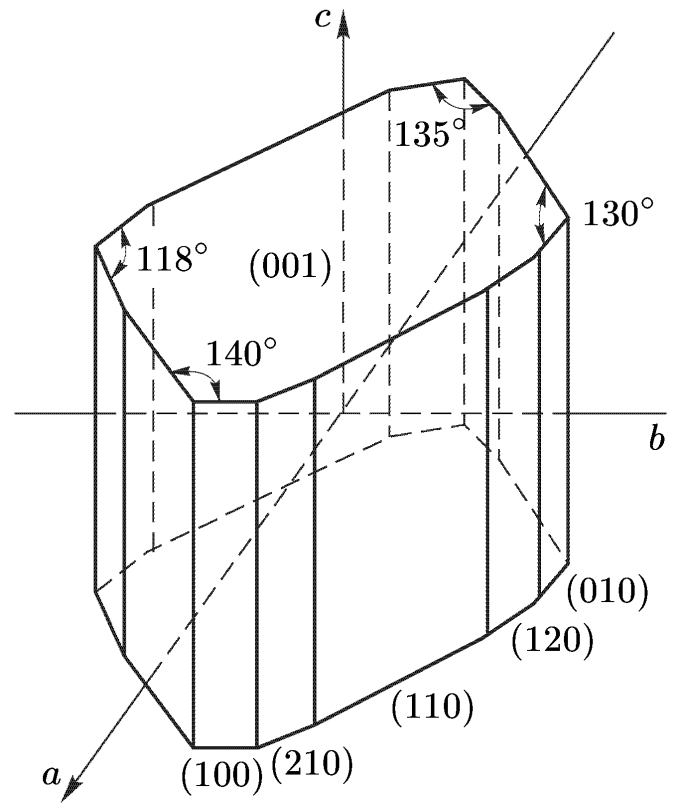
\includegraphics[width=0.38\textwidth]{soli.png}
    \end{wrapfigure}
    Будем иллюстрировать поведение сегнетоэлектриков на примере сегнетовой соли и титаната бария. В неполярной фазе (при $T< T_{\text{н}}$ и $T>T_{\text{в}}$) кристаллы сегнетовой соли относятся к ромбической системе и являются пьезоэлектриками. Наиболее развиты и типичны грани (001), а также призматические грани (110). Менее развиты грани (210), (120), (010). Грани (100) в большинстве случаев очень малы или совсем отсутствуют.
    В полярной фазе сегнетова соль принадлежит к моноклинной системе, причем полярная ось $a$ направлена параллельно исходной оси $a$ ромбического кристалла. Аномальные диэлектрические свойства сегнетовой соли выражены максимально, когда поле $E$ направлено по оси $a$. Аномалии не наблюдаются, когда направление $E$ параллельно осям $b$ и $c$.\\
    \\
    \textbf{Титанат бария}\\
\begin{wrapfigure}{l}{0.4\textwidth} % Картинка справа
    \centering
    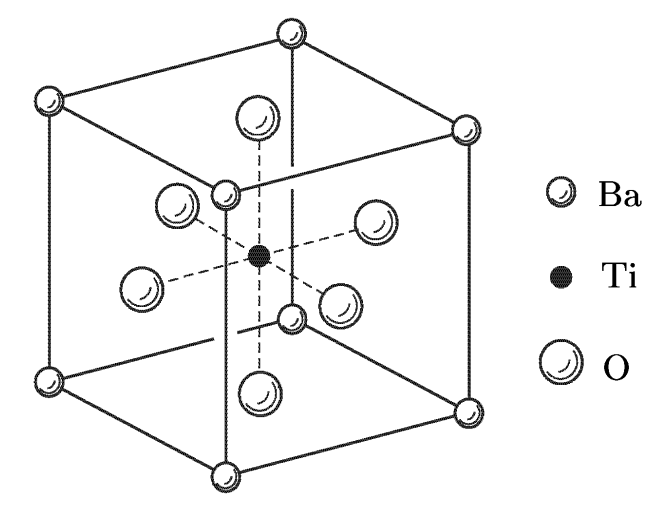
\includegraphics[width=0.38\textwidth]{TiBa.png}
\end{wrapfigure}
Теперь рассмотрим титанат бария.\\
В неполярной фазе выше 120°C это есть так называемая кубическая структура типа перовскита. Ввиду наличия центра симметрии титанат бария в неполярной фазе не обладает пьезоэлектрическими свойствами. В полярной области температур между точкой Кюри ($120 ^\circ C$) и температурой $5 ^\circ C$ кристаллы $BaTiO_3$ имеют тетрагональную симметрию и становятся пьезоэлектрическими. 

Фазовый переход при температуре $120 ^\circ C$ сводится к тому, что одно из ребер кубической ячейки удлиняется и становится полярной тетрагональной осью симметрии, обозначаемой через $c$, два других ребра одинаково укорачиваются, переходя в тетрагональные оси, обозначаемые через $a$. Какое из ребер исходной кубической ячейки удлинится и перейдет в полярную ось $c$ – дело случая. 

Однако если в результате флуктуации возникнет какое-то случайное удлинение, то оно определит выделенное направление, вдоль которого и будет происходить дальнейшее удлинение. Поскольку все три ребра кубической ячейки эквивалентны, каждое из них может перейти в полярную ось. В тетрагональной фазе существует шесть возможных направлений спонтанной поляризации – по два взаимно противоположных направления вдоль ребер кубической ячейки. 

Ниже $5^\circ C$ титанат бария испытывает второе фазовое превращение. Получается новая сегнетоэлектрическая фаза, устойчивая между $5$ и $-90^\circ C$ и обладающая орторомбической симметрией. Элементарная ячейка может быть получена из исходной кубической ячейки, если ее растянуть вдоль диагонали одной из граней куба и сжать вдоль другой диагонали той же грани. 

Растянутая диагональ служит полярной осью кристалла. Число граней и число их диагоналей – двенадцать. Однако эти диагонали попарно параллельны. Поэтому в орторомбической фазе существует двенадцать направлений, вдоль которых может ориентироваться вектор спонтанной поляризации кристалла. 

При $-90^\circ C$ происходит третий фазовый переход. Кристалл становится ромбоэдрическим с полярной осью вдоль одной из пространственных диагоналей куба, т.е. диагоналей, соединяющих его противоположные вершины. Так как исходная кубическая ячейка содержит четыре эквивалентных пространственных диагонали и каждой диагонали соответствуют два взаимно противоположных направления спонтанной поляризации, то в ромбоэдрической фазе существует восемь направлений, в которых может ориентироваться вектор спонтанной поляризации.

\section{Поляризация сегнетоэлектриков}
Рассмотрим поляризацию сегнетоэлектрика при наложении электрического поля. 
В полярной фазе она состоит из двух компонент: спонтанной поляризации $P_c$, которая от поля не зависит и индуцированной поляризации $P_\text{и}$.
Для начала стоит отметить, что связь между поляризацией и полем относится не к полной, а только к индуцированной поляризации. 
Связь между $P$ и $E$, в отличие от обычных диэлектриков нелинейна, поэтому обычные определения $\varepsilon$ и $\alpha$ не применимы. Исключением являются слабые поля, в которых все же можно ограничиться линейным приближением 
\[
P = P_c + P_\text{и}, 
\]
где $P_\text{и} = \alpha E$
В общем случае поляризуемость $\alpha$ является тензором, но если поле $E$ параллельно одной из трех главных осей тензора $\alpha$. В этом случае $\alpha$ является скаляром и можно вычислить по формуле 
\[
\alpha = \frac{\partial P_\text{и}}{\partial E}
\]
Диэлектрическая проницаемость: $\varepsilon = 1 + 4 \pi \alpha$

\section{Диэлектрическая проницаемость сегнетоэлектриков}
В полярной фазе значения диэлектрической проницаемости аномально велики, например для сегнетовой соли $\varepsilon \approx 10000$

В неполярной фазе сегнетоэлектрик ведет себя как обычный линейный диэлектрик, в котором поляризация пропорциональна электрическому полю. Однако поляризуемость $\alpha$ и диэлектрическая проницаемсть $\varepsilon$ меняются с температурой. Вблизи точки Кюри имеет место закон Кюри-Вейсса:
\[
\alpha = \frac{C}{T-T_0}, 
\]
где $C$ и $T_0$ - постоянные, из которых $T_0$ называется температурой Кюри-Вейсса(очень близка к температуре Кюри).
В случае, если точек Кюри две, то в окрестности каждой из них в неполярной фазе выполняется закон Кюри-Вейсса, в нижней в форме:
\[
    \alpha = \frac{C'}{T-T_0}, 
\]
Представлены температурные зависимости диэлектрической проницаемости монокристалла сегнетовой соли вдоль полярной оси $a$ и аналогичная кривая для титана бария. 
В орторомбической и тетрагональной фазах $\varepsilon$ измерена в тех же направлениях. В этих фазах кристалл разделяется на домены (см. ниже). С разделением на домены связано то обстоятельство, что кривые, снятые при возрастании и убывании электрического поля, в окрестности точек фазовых превращений не совпадают между собой.

\begin{minipage}{0.45\textwidth} % Левая картинка
    \centering
    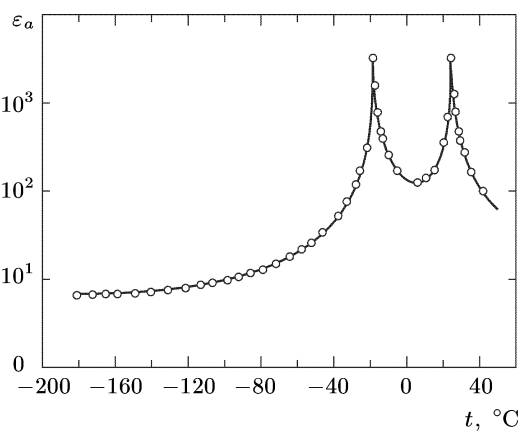
\includegraphics[width=\textwidth]{2.png}
    \textit{Рисунок 1. Описание первой картинки.}
\end{minipage}
\hfill
\begin{minipage}{0.45\textwidth} % Правая картинка
    \centering
    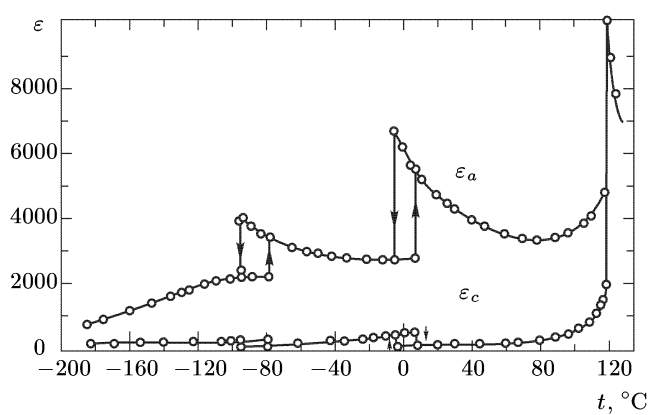
\includegraphics[width=\textwidth]{1.png}
    \textit{Рисунок 2. Описание второй картинки.}
\end{minipage}

\section{Петля гистерезиса}
\begin{wrapfigure}{l}{0.4\textwidth}
    \centering
    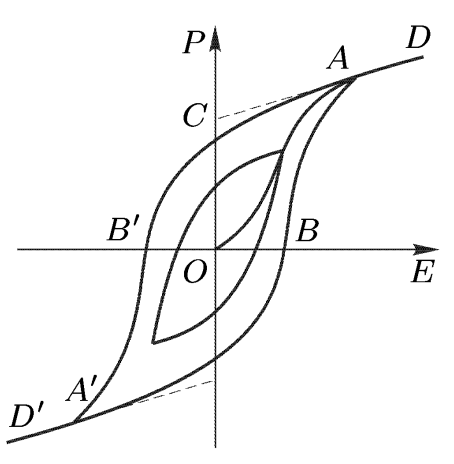
\includegraphics[width=0.38\textwidth]{gist.png}
\end{wrapfigure}
Благодаря доменной структуре дипольный момент кристалл сегнетоэлектрика равен нулю, так как поляризация одних доменов компенсиурется противоположно направленной поляризацией других. 
При наложении электрического поля происходит частичная переориентация доменов, а также рост одних доменов за счет других. 

Зависимость $P$ от напряженности электрического поля $E$ представлена на вдоль кривой OA. Сначала рост $P$ происходит вдоль кривой $OA$. В точке $A$ поляризация всех доменов оказывается ориентированной вдоль поля $E$. Начиная с этой точки, дальнейшее возрастание $P$ происходит за счет индуцированной поляризации $P_\text{и} = \alpha E$, и кривая OA переходит в прямолинейный участок AD. Если этот участок продолжить влево, то он отсечет на оси ординат отрезок $OC$, длина которого равна спонтанной поляризации $P_c$.

Будем теперь уменьшать напряженность электрического поля. Изменение поляризации пойдет на по прежней кривой, а по другой, расположенной выше. 

а по новой кривой $DAB'A'D'$, расположенной выше. Это явление называется диэлектрическим гистерезисом и связано с доменной структурой диэлектрика: процесс переориентации и роста доменов в электрическом поле задерживается, напоминая известное явление застоя,
обусловленное силами сухого трения. Таким образом, поляризация $P$ не определяется однозначно полем $E$, а зависит также
от предшествующей истории сегнетоэлектрика. Если менять электрическое поле в обратном порядке, то зависимость $P$ от $E$ изобразится нижней кривой $D'A'BAD$, симметричной с кривой $D'A'B'AD$ относительно начала координат О. Таким образом, получается замкнутая кривая $AB'A'BA$, называемая диэлектрической петлей гистерезиса. Можно получить петли гистерезиса меньших размеров, одна из кото- рых изображена на рис. 104. Совершенно аналогичные петли гистерезиса получатся, если по оси ординат откладывать индукцию $D = E + 4\pi P$. Они практически не отличаются (точнее, отличаются только масштабом) от кривых $P = P(E)$, так как в сегнетоэлектриках  $E < D$ слагаемым $E$ можно пренебречь.


\section{Микроскопические теории сегнетоэлектричества}
Предположим, что к диэлектрику с индуцированными диполями применимо выражение действующего поля $E' = E + \alpha P$, $\beta$ -- поляризуемость молекулы, $N$ -- концентрация. Тогда
\[
N \beta E' = P = N \beta E + N a \beta P
\]
\[
(1-N \alpha \beta)P = N \beta E
\]
если $Na\beta = 1$, то при $E = 1$ решениями уравнения будут $P = 0$ и $P \ne 0$. Из соответствующих им двух состояний реализуется то, что более термодинамически устойчиво. Тогда диэлектрик будет поляризован спонтанно: если сначала $\mathbf{P} = 0$, то всякая флуктуация поляризации $\mathbf{P}$ переводит диэлектрик в более устойчивое состояние, в котором $\mathbf{P} \neq 0$. Величина $N \alpha \beta$ зависит от температуры (хотя бы из-за теплового расширения диэлектрика). Условие $N \alpha \beta = 1$ определяет положение точки Кюри. В окрестности этой точки поляризуемость диэлектрика 
\[
\alpha = \frac{N \beta}{1 - N \alpha \beta}
\]
будет аномально велика. Разлагая знаменатель $1 - N \alpha \beta$ в ряд по степеням $T - T_k$ и ограничиваясь при этом линейным членом, придем к соотношению 
\[
\alpha = \frac{\text{const}}{T - T_k},
\]
т.е. к закону Кюри--Вейса. Данный пример показывает принципиальную возможность объяснения спонтанной поляризации и связанной с ней аномально большой величины $\varepsilon$ в окрестности точки Кюри.
\section{Применение сегнетоэлектриков на практике}

Конденсаторы с регулируемой ёмкостью используют нелинейную природу сегнетоэлектрических материалов. Обычно сегнетоэлектрический конденсатор или вариконд состоит из пары электродов, между которыми находится слой сегнетоэлектрического материала. Диэлектрическая проницаемость сегнетоэлектриков не только настраивается, но и обычно очень велика по абсолютной величине, особенно когда она близка к температуре фазового перехода. Благодаря этому сегнетоэлектрические конденсаторы имеют небольшой физический размер по сравнению с диэлектрическими (неперестраиваемыми) конденсаторами аналогичной ёмкости.

Наличие петли гистерезиса позволяет использовать эти материалы, в качестве функции памяти для изготовления сегнетоэлектрического RAM для компьютеров.
Комбинирование эффекта памяти, пьезоэлектричества и пироэлектричества делают сегнетоэлектрические конденсаторы очень полезными, например, для сенсорных приложений. Сегнетоэлектрические конденсаторы используются в медицинских ультразвуковых аппаратах (конденсаторы генерируют, а затем детектируют ультразвуковой сигнал, используемый для изображения внутренних органов тела), высококачественных инфракрасных камерах (инфракрасное изображение проецируется на двумерный массив сегнетоэлектрических конденсаторов, способных обнаружение разницы температур до миллионных долей градуса Цельсия), датчики огня, гидролокаторы, датчики вибрации и даже топливные форсунки в дизельных двигателях.


\begin{thebibliography}{99}
    \bibitem{author2024} Сивухин Д. В. Общий курс физики. 
    \bibitem{another2024} Another Author. Title of the Article. Journal Name, Volume(Issue), Year, Pages.
\end{thebibliography}
\end{document} 